% Graduation thesis
% Copyright 2016, Sjors van Gelderen

% Document settings
\documentclass{article}
\author{Sjors van Gelderen}
\title{Exploring advanced programming concepts}
\date{\today{}}

% Packages
\usepackage{amsmath}
\usepackage[utf8]{inputenc}
\usepackage{listings}
\usepackage{graphicx}
\graphicspath{{images/}}

% Content
\begin{document}

\maketitle{}

\newpage

\tableofcontents{}

\newpage

\section{Introduction}
In this document you will find a description of the materials I have studied during my graduation phase.
The primary focus of this project was to gain a greater understanding of data structures, algorithms and complexity analysis.
When studying these algorithms, I have focused primarily on worst case complexities. \huge why
Secondly, I was interested in gaining greater proficiency in the use of the Python 3 and C\# programming languages.
Lastly, I have taken a brief look at the C, Rust and Chicken Scheme programming languages. \huge why

\subsection{Languages}
Here I briefly describe the languages used to implement the concepts studied.

\subsubsection{Python 3}
Advantages of this language include its concise syntax and its portability.
Because of Python 3's high-level nature, the programmer can focus exclusively on the actual logic of the algorithm,
rather than the low-level memory management involved. This is removes a significant source of potential distraction.
A major downside of the language is the absence of a strict compiler.
Python programs frequently crash during run-time, as problems are not detected at compile-time.

\subsubsection{C\#}
With Microsoft's recent decision to join the Linux Foundation, the .NET platform is becoming ever more attractive.
The .NET platform is designed in such a way that its associated programming languages can directly interact with one another.
This brings to the programmer the possibility to combine multiple programming languages in a single project with great ease.
Since languages are designed with different problem-domains in mind, this offers increased expressive power to the programmer.
C\#, being perhaps the most popular .NET language, is an excellent choice to begin harnassing just this power.

\subsubsection{F\#}
Being a more recent addition to the .NET family of programming languages, F\# has not quite gained the popularity of C\#.
However, F\#'s conception has been a step along the way to many of the modern functional programming features incorporated in C\#.
F\# is an excellent and powerful multi-paradigm (though mostly functional) programming language.
Because of its functional nature, the F\# programming language enables the programmer to tackle problems using high-level concepts such as
recursion, higher order functions, partial application and currying, computation expressions (syntactic sugar for monads) and more.

\subsubsection{C}
Virtually any programmer will at some point in their career encounter this venerable, fast and portable programming language.
Because this low-level language doesn't use a garbage collector, the programmer must exercise great caution with the manual management of memory.
Many security problems that affect us today are a direct consequence of a failure to do so.
This language is interesting to one studying the low-level concepts of algorithms.

\huge Marked for appendix (rust / chicken scheme)
\subsubsection{Rust}
Developed by Mozilla, Rust aims to be a modern solution for safe, asynchronous programming.
With default immutable variables, as well as borrowing and lifetimes, the compiler makes it
very difficult indeed to write a program that contains run-time errors relating to incorrect memory access.

\subsubsection{Chicken Scheme}
The LISP family of programming languages has two major dialects; these being Common LISP and Scheme.
Chicken Scheme is a modern implementation of the Scheme dialect.
It has a very minimalistic syntax, revolving around the use of parentheses and prefix notation.
Chicken Scheme is a functional programming language.

\newpage

\section{Analysis}
\subsection{Empirical analysis}
Empirical analysis refers to inferring a program's expected performance based on measurements taken while running a program with various configurations.
A typical scenario involves the measurement of performance in terms of running time by the use of a 'stopwatch'.

\huge PROVIDE MINIMAL EXAMPLE WITH STOPWATCH IN C# HERE, USE INSERTION SORT AND PLOT GRAPH

\subsection{Complexity analysis}
Complexity analysis is different from empirical analysis in that it uses reasoning
- rather than experiment - to determine a program's expected performance.

\newpage

\section{Data structures}
As the manner in which data is stored affects the choice of algorithm,
it is appropriate to discuss the studied data structures now.

\subsection{Array}
Among the most common data structures for collections is the array.
All elements in the array are stored contiguously in memory,
and may be accessed in constant time(\(O(1)\)) through their respective indices.
Arrays have excellent cache-alignment, making them very fast indeed.

The location of an element in an array at some given index {\em i} will be
\[{\verb base_address_of_array } + i * s\]
In which {\em s} is the size of a single element.
This size depends on the data type of the array.

\subsubsection{Size}

\paragraph{Fixed size}
By default, arrays are generally of {\em fixed size}; meaning the array will take up constant space ({\em O(1)}).
Since less elements might be stored in the array than its total capacity allows for, space might be wasted on unused memory.
The amount of elements that are actually being used is called the {\em logical size} of the array.

\paragraph{Dynamic size}
When an array is of dynamic size, the programmer must carefully specify the amount by which the array will be resized.
If the programmer adds more elements than some given threshold will allow, the array must perform a resize operation.
Since the resize operation is costly (typically \(O(n)\)), it shouldn't occur too frequently.
In some implementations, dynamic size arrays will also shrink when the logical size becomes less than a given threshold.

\subsubsection{Dimensionality}
Arrays may have more than one dimension. Such a construction may also be called a matrix.
Elements in the multidimensional array may be accessed with multiple indices describing the relevant coordinates.


\subsection{Linked list}
The {\em linked list} is a linear, dynamic size data structure for storing collections of elements.
Contrary to arrays, elements are not guaranteed to be stored contiguously.
This makes it possible to store elements in a fragmented (non-contiguous) fashion,
which is useful when the collection is larger than any available contiguous block of memory.
Because of the fragmentation, elements cannot be accessed in constant time \((O(1))\) through the use of indices.

The linked list consists of several segments,
each of which has up to two references to other elements in the sequence.
Traversing the linked list is a linear time (\(O(n)\)) operation.

\paragraph{Singly-linked and doubly-linked}
The {\em singly-linked} list consists of segments that contain a value and a reference to the next segment in the sequence.
The {\em doubly-linked} list is the same as the singly-linked list, except each segment also has a reference to the previous segment in the sequence.
Whether the list is singly-linked or doubly-linked affects the traversal process,
since where singly-linked lists only allow forward traversal, doubly-linked lists also allow backward traversal.

\paragraph{Insert}
Inserting an element in the linked list requires traversing the list from start to end,
which is in the worst case a linear time (\(O(n)\) operation.
The last element will have a reference to a {\em null link}, meaning there is no next element in the sequence.
When this situation is encountered, the null link may be changed to refer to the new element instead.
If the list is {\em doubly-linked}, the new element's {\em previous} variable should reference the last element of the current list.

\paragraph{Delete}
The delete operation in the worst case requires a complete traversal of the list,
which is a linear time (\(O(n)\) operation. If the current element points to the element to be deleted,
the {\em next} reference must be changed to point to the element in the sequence that comes after the element to be deleted.


\subsection{Stack}
The {\em stack} is a {\em LIFO} (Last In, First Out) data structure.
The name of the data structure reveals its workings.
Data is always inserted on and removed from the top of the stack.
Only the top element of the stack may be inspected at any time.
Regardless of which structure is used to store the stack contents,
the interface must always offer the following operations: {\em push}, {\em pop} and {\em peek}.

\subsubsection{Implementation}
Here follows an example of a dynamic size stack implemented in Python 3.

\huge CHECK THIS BIT
\begin{lstlisting}[language=Python]
  class Stack:
    def __init__(self):
        self.contents = []

    def push(self, value):
        self.contents.append(value)

    def pop(self):
        self.contents.pop()

    def peek(self):
        if self.contents:
            return self.contents[-1]
        else:
            return None
\end{lstlisting}

\paragraph{Storage}
Storage is done using a Python 3 list.

\paragraph{Push}
The {\em push operation} puts a new element on top of the stack.
If the stack has a size limit, this operation might cause a {\em stack overflow} exception in the event that the stack's capacity is exceeded.

\paragraph{Pop}
The pop operation removes the top element from the stack. If the stack has no elements, this operation will throw an {\em stack underflow} exception,
as there are no elements left to remove.

\paragraph{Peek}
The peek operation gives the programmer access to the current top element of the stack.
If the stack is empty, this element may throw an {\em invalid operation} exception, as there are no elements to reveal.


\subsection{Queue}
Contrary to the stack, the queue is a {\em FIFO} (First In, First Out) data structure.
Elements are inserted at the back of the queue, and removed from the front of the queue.

\paragraph{Enqueue}
The {\em queue} operation removes the element at the front of the queue.


\paragraph{Dequeue}
The {\em dequeue} operation removes the element at the back of the queue.

\newpage

\huge MARKED FOR SCRAPPING
\subsection{Hashmap}
\subsubsection{Linear probing}
\subsubsection{Quadratic probing}
\subsubsection{Dynamic size buckets}

\newpage


\subsection{Tree}
Trees are hierarchical data structures consisting of {\em linked nodes}.
Unless the tree is empty, there will be a top node called the {\em root node}.
From this node spring all the {\em subtrees}.

Any node other than the root node of the tree is called a {\em child node}.
The predecessor of a child node is called its {\em parent}.
The root node is the only node that does not have a parent.

Nodes that don't have any children are called {\em leaves}, expanding on the analogy of the tree.

A tree is said to be {\em balanced} if the nodes are distributed evenly among the subtrees in the tree.
A tree might be so poorly balanced that the nodes are organized much like a {\em linked list}.
In this case, it's arguable that the tree was not a suitable data structure for the relevant problem.


parents

leafs

levels

\subsubsection{Binary tree}
The binary tree consists of nodes containing at most one parent, and at most two children.
There is no particular property governing where new elements are inserted.
This is because the binary tree does not inherently imply any particular sorting order.

\subsubsection{Heap}
This binary tree maintains the {\em heap property}, which is said to be {\em max} or {\em min}.
A heap that satisfies the {\em max heap property} is called a {\em max heap}.
Accordingly, a heap that satisfies the {\em min heap property} is called a {\em min heap}.
The property determines the order in which the elements are stored inside the heap.

For example, in a max heap each key must be greater than every key stored inside its children.
Conversely, in a min heap each key must be less than every key stored inside its children.

\paragraph{Heapify}
The heapify operation will help us maintain the heap property on our data.

\begin{lstlisting}[language=Python]
  def heapify(index):
        c = self.keys
        left = get_left_child_index(index)
        right = get_right_child_index(index)
        largest = index

        property_holds = c[left] > c[index] if self.max else c[left] < c[index]
        
        if left <= self.heap_size and property_holds:
            largest = left

        property_holds = c[right] > c[largest] if self.max else c[right] < c[largest]
        
        if right <= self.heap_size and property_holds:
            largest = right
        
        if largest != index:
            swap(index, largest)
            heapify(largest)
\end{lstlisting}

\paragraph{Build}
This simple operation takes as input a collection of elements of which the heap will consist.
Since we have already defined a means of enforcing the heap property, we may simply use that same logic to construct the tree.

\begin{lstlisting}[language=Python]
  # INCORRECT PLEASE FIX
  def build(self, collection):
    for element in collection:
      self.heapify(len(self.keys) - 1)
\end{lstlisting}

\subsubsection{Binary search tree}
Contrary to the regular binary tree, the binary search tree must satisfy an ordering principle.
This principle is known as the binary tree property. Thanks to this property,
more efficient searching algorithms are possible.

\subsubsection{K-dimensional tree}
The K-dimensional tree expands upon the philosophy of the binary search tree, in that it
must maintain a sorting order property. When using this tree in less than 3 dimensions,
a simple geometric interpretation of its structure is possible.

\paragraph{Construction}
Let's examine the construction of a 2-dimensional tree from the array \(A = [(3, 2), (6, 5), (7, 1)]\).
The root key of the tree will be the first element in the array, in this case (3, 2).
We will record this key as a {\em vertical} split of the plane, like so:

{\huge INSERT GRAPHIC HERE}

Since the next key in the collection - (6, 1) - has a larger {\em X} coordinate than the root key(\(6 > 3\)), it will be stored to the left of the root key.

Notice that this operation has added a new level to our tree. In a 2-dimensional tree, each level of the tree will be recorded as being either {\em vertical} or {\em horizontal}.

For this example, let's assume that even levels are {\em vertical}, whereas odd levels are {\em horizontal}.

The next key in our collection - (7, 1) - has a larget {\em X} coordinate than our root key(\(7 > 3\), so the key must be stored in the right subtree. However, the right subtree is not empty, and so we must compare the right child of the root key to the key from our insertion collection. Since the right child of the root key is on an odd level in our tree, it corresponds to a {\em horizontal} split. The consequence of this difference is that we must now compare the {\em Y coordinates} rather than the {\em X coordinates} of our keys. Since the {\em Y} coordinate of our insertion key is less than that of the right child of the root key, we must store our new element to the left the right child of the root key.

\newpage

\subsection{Graph}

\subsubsection{Adjacency list}


\subsubsection{Adjacency matrix}
\subsubsection{Incidence matrix}

\newpage

\section{Algorithms}
\subsection{Searching}
\subsubsection{Linear search}
The linear search is a very simple algorithm. It linearly traverses a collection until either the requested
element is found, or the end of the collection was reached.

\subsubsection{Binary search}
If the collection is known to be sorted, binary search may yield a significant performance gain over regular insertion sort.

\newpage

\subsection{Sorting}
\subsubsection{Insertion sort}


\subsubsection{Shell sort}

\subsubsection{Comb sort}

\subsubsection{Radix sort}

\subsubsection{Counting sort}

\subsubsection{Bucket sort}

\subsubsection{Heap sort}

\subsubsection{Merge sort}
This sorting algorithm splits a collection into many small collections.
Each of these small collections is sorted and subsequently merged with another small collection.
Eventually this algorithm yields a sorted collection faster than a regular insertion sort.

\subsubsection{Quick sort}
Via the use of a pivot, the collection is divided and subsequently conquered.

\subsubsection{Monkey sort}
Imagine having an unsorted deck of cards, then throwing it in the air and picking it up to see if the new distribution is sorted.
If it's not, then you repeat the process. This is a quaint description of {\em Monkey sort}.
It's a highly inefficient sorting algorithm, in which a random distribution of the collection is made every time.
Subsequently, the new distribution goes through a process that verifies if it is sorted. If it is not sorted, a new distribution is made.
Since this algorithm may never yield a sorted distribution, the complexity is unbounded ($O(\infinity)$).

\newpage

\subsection{Shortest path determination}
In this section, each of the following algorithms is assumed to operate on the following graph:

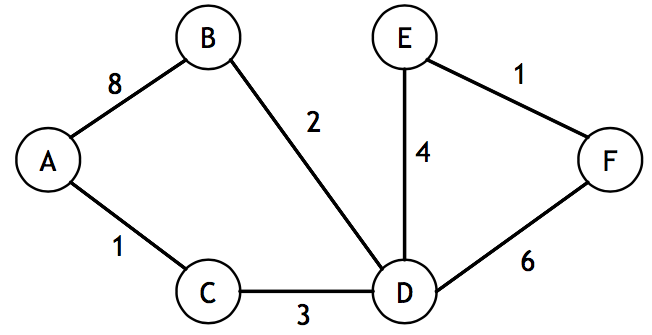
\includegraphics[width=\textwidth]{sample_graph}

When recording this graph as data, letters are replaced with 0-based indices, such that \(A=0, B=1, C=2, \dots\). The graph is said to consist of a set of {\em vertices}, \(V\) and a set of {\em edges}, \(E\). Vertices may be connected to one another through one or more edges. Such a connection is called a {\em path}.
The bar-notation is used to indicate the amount of elements in a set, such that \(|V|\) is the amount of vertices and \(|E|\) is the amount of edges.

\subsubsection{Dijkstra}
This algorithm finds all shortest path distances between a source vertex and all other vertices in a graph.
With a slight modification it becomes possible to also track the actual paths, rather than just the distances.

Obviously Dijkstra requires a graph, so let us construct one.
In my implementation, I have created two classes:

\begin{lstlisting}[language=Python]
# Edge connected to a node in a graph
class Edge:
    def __init__(self, target_id, distance):
        self.target_id = target_id
        self.distance = distance

# Vertex in a graph
class Node:
    def __init__(self, id):
        self.id = id
        self.edges = []
\end{lstlisting}

Next, we need a simple way to specify connections between vertices.

\begin{lstlisting}[language=Python]
# Connect two nodes
def connect(node_0, node_1, distance):
    if node_0 != node_1 and \
       node_1 not in node_0.edges and \
       node_0 not in node_1.edges:
        node_0.edges.append(Edge(node_1.id, distance))
        node_1.edges.append(Edge(node_0.id, distance))
\end{lstlisting}

Using these constructs, we may build the final graph as follows:

\begin{lstlisting}[language=Python]
  # Build the graph and weighted paths
    graph = [ Node(id) for id in range(6) ]
    
    connect(graph[0], graph[1], 8)
    connect(graph[0], graph[2], 1)

    connect(graph[1], graph[3], 2)

    connect(graph[2], graph[3], 3)

    connect(graph[3], graph[4], 4)
    connect(graph[3], graph[5], 6)

    connect(graph[4], graph[5], 1)
\end{lstlisting}

\subsubsection{Floyd-Warshall}
Rather than Dijkstra's focus on a single source, Floyd-Warshall finds the shortest path between each vertex and all other vertices in a graph. In addition, it supports negative weights for the edges in the graph.

Initially, one might suspect that this algorithm somehow runs Dijkstra on each vertex.
This would be rather inefficient. Fortunately, Floyd-Warshall uses a more clever approach.

To get started, we'll need to construct a graph and specify the weight of each edge.
Python 3 allows us to record exactly this using a concise syntax:

\begin{lstlisting}[language=Python]
  graph = {
    0: {1: 8. 2: 1},
    1: {0: 8, 3: 2},
    2: {0: 1, 3: 3},
    3: {1: 2, 2: 3, 4: 4, 5: 6},
    4: {3: 4, 5: 1},
    5: {3: 6, 4: 1}
  }
\end{lstlisting}

Which is essentially a weighted adjacency list which we will supply to the Floyd-Warshall algorithm to generate our final result.

Now we set up the initial 'guess' of our algorithm.
The first step is to set up a matrix of distances between vertices.
Initially, this matrix will contain the value infinity for each distance.
In my implementation, I've used a multidimensional list comprehension to generate this matrix:

\begin{lstlisting}[language=Python]
  distances = [
    [
      0 if x == y else inf \
      for x in range(len(graph)) \
    ] \
    for y in range(len(graph))
  ]
\end{lstlisting}

Then, we populate our matrix with a slightly better guess, containing the distances between vertices of just that share an edge.

\begin{lstlisting}[language=Python]
    for vertex, connections in graph.items():
        for target, distance in connections.items():
            distances[vertex][target] = distance
\end{lstlisting}

Finally, we must run the actually interesting part of the algorithm.
This part is also what primarily defines the complexity class of this algorithm's running time.

\begin{lstlisting}[language=Python]
  for k in range(len(graph)):
        for i in range(len(graph)):
            for j in range(len(graph)):
                if distances[i][j] > distances[i][k] + distances[k][j]:
                    shorter_distance = distances[i][k] + distances[k][j]
                    print("Improving {} -> {} from {} to {}"
                          .format(i, j, distances[i][j], shorter_distance))
                    distances[i][j] = shorter_distance
\end{lstlisting}

We have three {\em for} loops, using the variables {\em i}, {\em j}, and {\em k}.
At each point, {\em i} and {\em j} are always two vertices between which we are trying to find the shortest path. The most interesting part of the algorithm actually relies on {\em k}.

{\em k} at each iteration represents a vertex between {\em i} and {\em k}, which may potentially yield a shorter path from {\em i} to {\em j}. This means that each time we find a shorter path, we'll have to update the currently recorded value in our distance matrix.

Since we have three {\em for} loops that each scale according to the amount of vertices in the graph,
it naturally follows that the complexity class of our algorithm is \(O(n^3)\).

\newpage

\section{Advanced C\# features}
\huge MARKED FOR SCRAPPING
\subsection{Properties}
This concept allows the programmer to specify how data inside a class may be accessed.
With this feature, manually writing {\em get} and {\em set} functions becomes obsolete.

{\huge FURTHER EXPLANATION REQUIRED}

\subsection{Interfaces}
Interfaces are contracts that guarantee a class implements certain methods.

\subsection{Events}
Event-driven programming is made possible in C\# through the use of {\huge UNFINISHED SENTENCE}.

\subsection{Extension methods}
In order to extend the functionality offered by base types, a programmer may use extension methods.

\subsection{Lambdas, delegates and higher order functions}
Higher order functions are part of what makes functional programming so powerful.
In C\#, delegates and lambdas offer the features required for higher order functions.

Here are several examples of how these concepts may be applied.

\paragraph{Iter}
This operation iterates over a sequence of elements. For each of these elements the provided lambda will be executed.

\begin{lstlisting}[language=Python]
  // This function prints all elements in the collection
  List.iter (fun element -> printfn "%A" element) collection
\end{lstlisting}

\paragraph{Filter}
This operation iterates over a sequence of elements. For each of these elements, the provided lambda predicate will be executed.
Elements for which this predicate returns True will be in the resulting list. Contrastingly, elements for which the predicate returns False will be discarded.

\begin{lstlisting}[language=Python]
  // This function returns all elements in the collection that are even
  List.filter (fun element -> element % 2 == 0) collection
\end{lstlisting}

\paragraph{Map and reduce}
This operation iterates over a sequence of elements. For each of these elements, the provided lambda will be executed.
The lambda contains a function that manipulates the current element. The result of this operation is the list of transformed elements.

\begin{lstlisting}[language=Python]
  //This function returns all transformed elements in the collection
  List.map (fun element -> element + 4) collection
\end{lstlisting}
  
\paragraph{Fold}

\paragraph{LINQ}


\subsection{Anonymous types}
Using this feature, programmers may easily specify new types with a comfortable syntax.

\begin{lstlisting}[language=Python]
  var some_type = { SomeProperty = 5 };
\end{lstlisting}

\subsection{Iterators and state machines}


\subsection{Indexers and enumerators}

\newpage

\section{Asynchronous programming}
\subsection{Async and await}
\subsection{Coroutines}
\subsubsection{The coroutine monad}
\subsection{Threading}

\newpage

\section{Design patterns}

\subsection{Option and Visitor}
These design patterns when combined form a great answer to the infamous null-reference-exception.
In essence, the {\em option} pattern offers a syntactical construct that forces the programmer to deal with missing data at {\em compile time}.
Data in the option is said to be either {\em some data} or {\em none}, the latter of which replaces the traditional {\em null}.
Since {\em none} is {\em no data} rather than {\em missing data}, a null-reference-exception shan't occur.

The option's counterpart is the {\em visitor}, which offers a syntactical construct to perform different operations depending on whether data
is missing({\em none}) or readily available ({\em some data}).

The following example demonstrates this process:

\huge SECTION INCOMPLETE, REPLACE WITH C# DESIGN PATTERN
\begin{lstlisting}[language=Python]
\end{lstlisting}

The two variables({\em noneData} and {\em someData}) are defined to be of type {\em Option String}.
That is to say, the variables may either hold actual data({\em some}) or not{\em none}.
When interacting with {\em Option} data, the programmer must use a {\em match} expression.
Such an expression is forced by the compiler to deal with both possible cases({\em some} and {\em none}.
Notice how {\em some} comes with a {\em data} object, {\em none} does not.

\subsection{Factory}
\subsection{Strategy}
The strategy pattern is used where different strategies may be optimal depending on context.
For instance, if we know a collection to be mostly sorted, we might choose to use a different sorting algorithm than when the collection is mostly unsorted.

\huge SECTION INCOMPLETE, PROVIDE C# CODE HERE

\subsection{Adapter}
Programmers will frequently encounter situations in which they must deal with error-prone code.
For example {\huge C# EXAMPLE HERE}.
Unfortunately, one is frequently not allowed to modify existing code.
To deal with this situation efficiently, the programmer may employ a technique called the {\em adapter pattern}.
The adapter pattern consists of building a new interface to existing code.
The primary purpose of this new interface is to guarantee proper interaction with the existing code.

\newpage

\section{Conclusion}


\section{Bibliography}


\end{document}
